\documentclass[Orbiter User Manual.tex]{subfiles}
\begin{document}

\subsection{Space Shuttle Atlantis}
\label{ssec:atlantis}
Space Shuttle Atlantis, comprising the complete launch stack of orbiter, external tank and solid rocket boosters, represents the only "real" spacecraft in the basic Orbiter distribution - but there are many more available as add-ons. Its flight characteristics and fuel management are less forgiving than fictional models like the Delta-glider, and much of it (esp. the launch phase) is automated to ease pilot workload.

\alertbox{Make sure to activate \textit{Limited fuel} in the Parameters tab of the Launchpad dialog before flying the Space Shuttle. Without consuming fuel, Atlantis is too heavy to reach orbit.}

\begin{figure}[H]
	\centering
	\subfigure{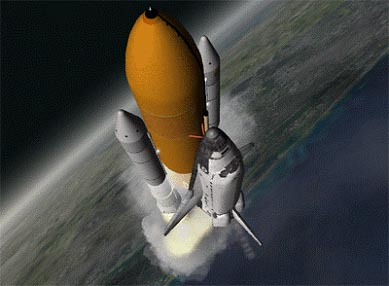
\includegraphics[width=0.75\textwidth]{atlantis.jpg}}
	\caption{Atlantis 3D model and textures: Michael Grosberg, Don Gallagher (orbiter) and Damir Gulesich (ET+SRB). Original module code: Martin Schweiger. Original grappling, RMS and MMU extensions: Robert Conley. Module code extensions: David Hopkins and Douglas Beachy.}
\end{figure}

\noindent
The Atlantis orbiter features a virtual cockpit with working MFD instruments and head-up display, and an operational payload bay with remote manipulator arm ("Canadarm"), so the deployment or even recapture of satellites can be simulated, as well as the shipment of resupplies to the International Space Station. Also included is MMU (manned manoeuvring unit) support for extravehicular activities.


\subsubsection{Virtual cockpit}
You can switch between generic glass cockpit view and virtual cockpit (VC) by pressing \keystroke{F8}. The virtual cockpit puts you directly on the Atlantis flight deck into the commander's, pilot's or payload specialist's seat, surrounded by display screens and instrument panels. Currently, a subset of instruments is active, including 10 working MFDs, and panel R13L in the rear of the flight deck, controlling the payload door operations.

\begin{center}
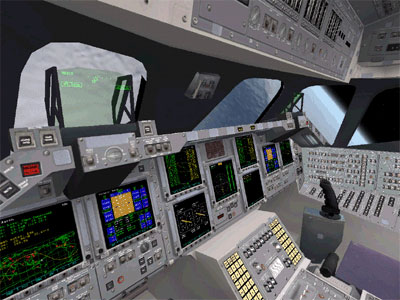
\includegraphics[width=0.75\textwidth]{atlantis_vc.jpg}
\captionof{figure}{The virtual cockpit from the commander's seat}
\end{center}

\paragraph{Navigating the VC}
There are three camera positions available: commander, pilot and payload specialist. By default, you are placed in the commander's seat, but you can move to a different position by pressing \keystroke{Ctrl} and an arrow key.  \keystroke{Ctrl}\keystroke{$\rightarrow$} and \keystroke{Ctrl}\keystroke{$\leftarrow$} jump between the commander and pilot seats, while \keystroke{Ctrl}\keystroke{$\downarrow$} switches to and from the payload operator position.\\

\noindent
\textbf{Looking around}\\

\noindent You can rotate the view at each of the three positions in different ways:
\begin{itemize}
\item by pressing Alt and a cursor key
\item by pressing the right mouse button and dragging the mouse
\item by using the direction controller on the joystick, if available 
\end{itemize}
\vspace{0.5cm}
\noindent
\textbf{Leaning forward and sideways}\\

\noindent
You can also move the head position by pressing \keystroke{Ctrl}\keystroke{Alt} in combination with a cursor key. Leaning forward \keystroke{Ctrl}\keystroke{Alt}\keystroke{$\uparrow$} in the commander or pilot position will get you closer to the HUD and instrument panels. Leaning sideways (\keystroke{Ctrl}\keystroke{Alt}\keystroke{$\rightarrow$} and \keystroke{Ctrl}\keystroke{Alt}\keystroke{$\leftarrow$}) provides better access to the MFD instruments on the central panel, or give a better view out of the windows.
In the payload operator position, \keystroke{Ctrl}\keystroke{Alt}\keystroke{$\rightarrow$} provides a view out of the right payload bay window, \keystroke{Ctrl}\keystroke{Alt}\keystroke{$\uparrow$} gets you close to one of the top windows, and \keystroke{Ctrl}\keystroke{Alt}\keystroke{$\leftarrow$} brings the payload door operation panel (R13L) into view.
In all positions, \keystroke{Ctrl}\keystroke{Alt}\keystroke{$\downarrow$} returns to the default head position.

\paragraph{Operating the MFDs}
The VC provides 10 multifunctional displays which can be operated independently:
\begin{itemize}
\item 2 commander MFDs (CDR1 and CDR2), accessible from the commander position
\item 2 pilot MFDs (PLT1 and PLT2) accessible from the pilot position
\item 5 MFDs on the central console, accessible from commander and pilot positions
\item 1 MFD on the right rear panel, accessible from the payload operator position
\end{itemize}
Due to the layout of the Shuttle MFD control switches, the operation differs slightly from the generic Orbiter MFD setup. All 10 MFDs work identically. The controls consist of a power button on the left, a brightness dial on the right, and 6 function buttons along the bottom edge.
\begin{itemize}
\item Clicking the power button turns the MFD on and off.
\item Clicking the left and right half of the brightness button decreases and increases the display brightness, respectively.
\item The left 5 function buttons provide mode-specific functions. The corresponding labels displayed at the bottom of the display change accordingly.
\item The right function button (PG) has a double function: Clicking briefly pages through the function buttons, if the current mode supports more than 5 functions. Holding down the button for longer than one second brings up the mode selection page, with 5 entries per page. You can use the function buttons to select one of the modes.
\end{itemize}
\begin{center}
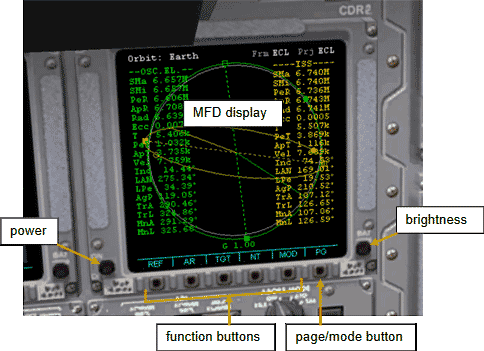
\includegraphics[width=0.75\textwidth]{atlantis_mfd.png}
\captionof{figure}{Shuttle MFD screen.}
\end{center}

\subsubsection{Notes on operation}
This section contains some details on launch, docking and payload operations of the default Atlantis model distributed with Orbiter. To test the procedures described here in practice, launch Orbiter and try any of the scenarios in the Space Shuttle Atlantis folder.

\paragraph{Launch autopilot}
The Space Shuttle needs to follow a tightly defined ascent profile to reach a stable orbit with the available fuel resources, in particular when transporting a heavy payload, or if the mission requires a a high or inclined orbit. You are free to try it manually (unlike the real shuttle), but it is easier (and more realistic) to leave the launch and ascent to the automatic systems.\\

The interface to the ascent autopilot is implemented as an MFD mode (AscentAP, \keystroke{Shift}\keystroke{B}). The AP mode has four pages which can be cycled with the \texttt{PG-} and \texttt{PG+} buttons. Only the first two pages are currently implemented.\\

Page 1 is the AP configuration page where some of the target orbit parameters can be specified before launch. The launch azimuth angle can be adjusted with the \texttt{AZ-} and \texttt{AZ+} buttons. The selected azimuth, as well as the resulting orbit inclination, are displayed on the page. When launching from Cape Canaveral, the allowed launch azimuth range is 35°-120°, although in practice the Shuttle always launched in north-eastern direction. Remember that the further you deviate from a western (90°) azimuth, the less the trajectory will benefit from Earth's rotation in terms of initial velocity, and the tighter your fuel budget will be. If the mission calls for a very inclined orbit, you may not be able to load the Shuttle to full payload capacity (30t).\\

The second configurable parameter is the target orbit altitude, adjusted with \texttt{AL-} and \texttt{AL+}. Reaching higher orbits requires more fuel, so if you specify a higher orbit than can be achieved with the available fuel load, the engines will cut out before the trajectory reaches the target apoapsis distance, and there won't be any reserves for the orbit circularisation burn.\\

Finally, you can schedule or skip the OMS-2 burn. OMS-2 is the second burn of the shuttle orbiter's OMS (Orbital Maneuvering System) engines. Its purpose is to circularise the orbit once the spacecraft reaches the apoapsis point during ascent. OMS-2 can be commanded to be performed automatically, or you can disable it and then manually perform any required circularisation maneuvers. If the OMS-2 burn is disabled, the AP will disengage at the end of the OMS-1 burn, when the apoapsis distance has reached the commanded orbit altitude.\\ 

\begin{center}
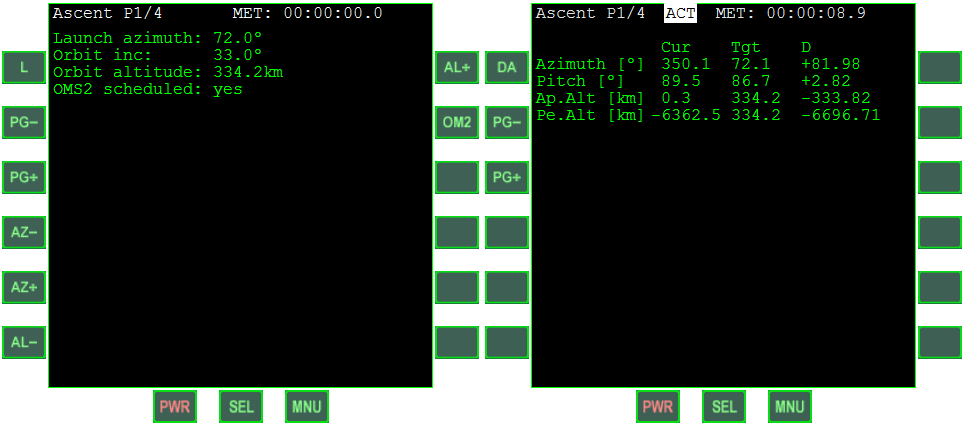
\includegraphics[width=\textwidth]{atlantis_ascent_ap_1.png}
\captionof{figure}{Ascent AP pre-launch configuration page (left) and parameter monitoring page (right).}
\end{center}

Once all launch parameters have been set and the launch window has opened, press L to commence the launch sequence. This will start with the space shuttle main engine (SSME) ignition, and once thrust has stabilised, followed by solid rocket booster (SRB) ignition, and the release of the hold-down bolts.
After lift-off the first page of the AP display switches to monitoring mode, where the target and current values of azimuth, pitch, apoapsis and periapsis altitude are shown as well as the differences.\\

During the first phase of the launch, the stack's attitude in pitch, yaw and roll is controlled by thrust-vectoring both the SSMEs and the SRB engines. The current gimbal positions of all engines are shown on page 2 of the AP display. The engine mounts allow rotation in both the yaw and pitch axes to provide pitch, yaw and bank moments for the launch stack (while the SRBs are attached, the SSME engines only gimbal in pitch, while the yaw axis is disabled).\\

\begin{center}
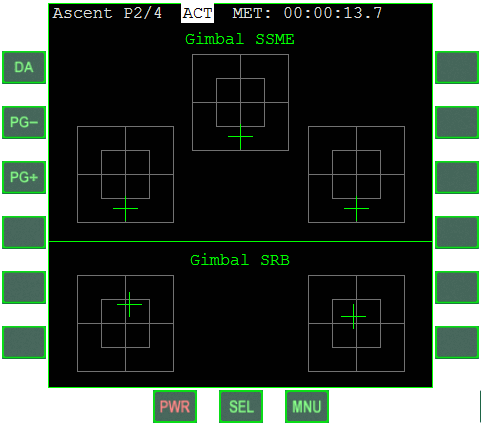
\includegraphics[width=0.5\textwidth]{atlantis_ascent_ap_2.png}
\captionof{figure}{SSME and SRB gimbal monitor.}
\end{center}

After SRB separation, the remaining orbiter + ET (external tank) assembly performs a "rotate upright" maneuver - a rotation of 180° around the longitudinal axis. This is initiated and terminated by a differential pitch gimbal position of the two outer SSMEs.\\

After SSME cut-off and the separation of the ET, attitude control switches to the RCS (reaction control system) - a set of small thrusters engaged in pairs to provide moments around the orbiter's three axes. These align the orbiter for the OMS-1 burn, using the two OMS engines powered by the on-board fuel supply. The OMS-1 burn commences automatically if the AP is active, and terminates once the apoapsis altitude matches the commanded orbit radius.\\

If the OMS-2 burn was disabled, the AP disengages at this point. Otherwise, the AP waits until the apex of the orbit is reached, then re-aligns the orbiter attitude and fires the OMS engines again to raise periapsis altitude until the orbit is circular with the commanded radius. OMS is cut off and the AP disengages.
You can disengage the AP at any point during the ascent by pressing the DA button on the MFD. This should only be done in an emergency!

\paragraph{Manual launch}
You are welcome to ignore the launch autopilot and try to fly the ascent profile manually (a challenge not offered to the real Shuttle pilots). To launch, engage the SSMEs at 100\% thrust (\keystroke{Num+} and \keystroke{R-Ctrl} to lock). The SRB engines ignite automatically, the hold-down bolts are blown off, and the launch stack will lift off from the pad. You can control the assembly's attitude with the normal maneuvering controls (joystick and keyboard, see \ref{sec:controls} for details). The pilot's attitude commands are translated to gimbal deflections of the SSMEs and SRB engines. You can monitor the gimbal positions on page 2 of the ascent autopilot (see previous section). The gimbal information on that page works even when the autopilot is not active. Make sure that the RCS is not activated during ascent. Attitude control during the early flight phase is by thrust-vectoring only.\\

At T + 2:06 minutes (126 seconds after ignition), the SRB fuel is spent and the SRBs detach automatically. In an emergency you can jettison the SRBs early \keystroke{J}, but in that case you probably also want to jettison the ET (\keystroke{J} again) and try to return the orbiter to the runway.\\

The following phase of the ascent is flown with the SSMEs only, fed from the ET. As fuel is consumed, the assembly becomes lighter and acceleration increases. Throttle down to keep acceleration at 3g.\\

At T+8:58 minutes, the ET is empty and separates automatically (or can be separated manually before that with \keystroke{J}). Altitude at this point should be approximately 110km.\\

After tank separation, the orbiter's throttle controls now address the OMS engines, fed from internal fuel tanks. Use the initial OMS burn (OMS-1) to push the trajectory apoapsis to the target orbit altitude. Then cut OMS, wait until the Shuttle reaches apoapsis, and fire again prograde (OMS-2) to circularise the orbit. If you flew a good ascent profile, you won't have run out of fuel yet, and still have enough for the deorbit burn. Otherwise, you are in trouble.\\

\paragraph{Docking}
The Shuttle orbiter can carry a docking attachment in the cargo bay. In the real shuttle this was only installed if the mission required docking (e.g. to the ISS), but removed otherwise as it limits payload capacity. In Orbiter, the docking attachment is permanently installed.\\

Prior to docking, the cargo bay doors must be fully open. The docking approach direction is upward as seen from the shuttle orbiter (+y). The Docking MFD mode can be used for linear and rotational alignment, but the relationship between RCS commands and the resulting acceleration axes is different to nose-mounted docking ports and must be considered carefully.

\begin{center}
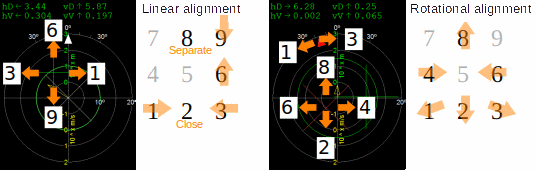
\includegraphics[width=0.75\textwidth]{atlantis_dock.png}
\captionof{figure}{Effect of RCS command input on linear/rotational alignment cues in Docking MFD for Shuttle with docking adapter installed in cargo bay.}
\end{center}

\subsubsection{Payload bay operations}

The payload bay operations in Orbiter's Atlantis implementation consist of
\begin{itemize}
\item opening and closing the payload bay doors
\item deploying and retracting the forward radiator panels
\item deploying and retracting the Ku-band antenna
\item operating the RMS arm for deploying and stowing payload
\end{itemize}

\noindent
The bay doors, radiators and Ku-band antenna operation closely follows the real shuttle procedures, using panel R13L. This panel is accessible from the payload operator position of the VC (via \keystroke{Ctrl}\keystroke{Alt}\keystroke{$\leftarrow$}). Alternatively, a dialog representation of the panel is available by pressing \keystroke{Ctrl}\keystroke{Space} and selecting Payload door operation. The dialog is also available in external views.

\begin{center}
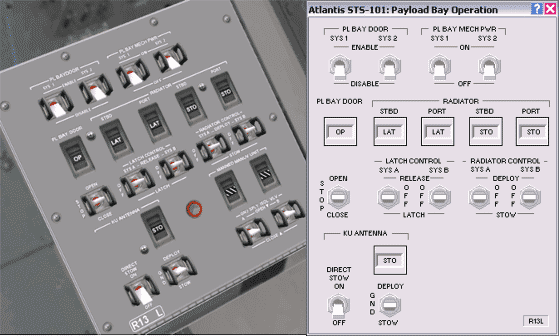
\includegraphics[width=0.75\textwidth]{atlantis_r13l.png}
\captionof{figure}{Panel R13L in the virtual cockpit (left) and as a dialog (right).}
\end{center}

\paragraph{Bay door operation}
\label{para:atlantis_baydoor}

\textbf{Bay door opening sequence:}
\begin{itemize}
\item Set the PL BAY DOOR switch to STOP.
\item Set the PL BAY DOOR SYS 1 and SYS 2 switches to ENABLE.
\item Set the PL BAY DOOR switch to OPEN.
\item Wait until the OP/CL status of the talkback indicator shows OP.
\item Set the PL BAY DOOR switch to STOP.
\item Set the PL BAY DOOR SYS 1 and SYS 2 switches to DISABLE.
\end{itemize}

\noindent
\textbf{Bay door closing sequence:}
\begin{itemize}
\item Make sure that the radiators, Ku-band antenna and RMS arm are stowed.
\item Set the PL BAY DOOR switch to STOP.
\item Set the PL BAY DOOR SYS 1 and SYS 2 switches to ENABLE.
\item Set the PL BAY DOOR switch to CLOSE.
\item Wait until the OP/CL status of the talkback indicator shows CL.
\item Set the PL BAY DOOR switch to STOP.
\item Set the PL BAY DOOR SYS 1 and SYS 2 switches to DISABLE.
\end{itemize}

\paragraph{Radiator operation}
The Space Shuttle has four radiators to dissipate heat from the coolant loops - two on the inside of each of the payload bay doors. The forward radiator panels on each side can be deployed when the doors are open; the aft panels are fixed. The radiator deployment is also controlled from panel R13L.\\

\noindent
\textbf{Radiator deployment sequence:}
\begin{itemize}
\item The payload bay doors must be fully open.
\item Set the PL BAY MECH PWR SYS 1 and SYS 2 switches to ON.
\item Set the LATCH CONTROL SYS A and SYS B switches to REL (release).
\item After 30 seconds, set both latch control switches back to OFF.
\item Set the RADIATOR CONTROL SYS A and SYS B switches to DEPLOY.
\item After 50 seconds, set both radiator control switches back to OFF.
\item Set both PL BAY MECH PWR switches back to OFF.
\end{itemize}

\noindent
\textbf{Radiator stowing sequence:}
\begin{itemize}
\item Set the PL BAY MECH PWR SYS 1 and SYS 2 switches to ON.
\item Set the RADIATOR CONTROL SYS A and SYS B switches to STOW.
\item After 50 seconds, set both radiator control switches back to OFF.
\item Set the LATCH CONTROL SYS A and SYS B switches to LATCH.
\item After 30 seconds, set both latch control switches back to OFF.
\item Set both PL BAY MECH PWR switches back to OFF.
\end{itemize}

\paragraph{Ku-band antenna operation}
\label{para:atlantis_antenna}
The Ku-band antenna is carried on the starboard sill longeron inside the orbiter's cargo bay and can be deployed once the payload bay doors are open. The antenna is used for communication with ground stations. Alternatively, it can also be used as a radar system for tracking objects in space. The controls for deployment and stowage of the Ku-band system are located on panel R13L. Jettisoning the assembly, and the actual functionality of the Ku-band system are not currently implemented in this version.\\

\noindent
\textbf{Ku-band deployment sequence:}
\begin{itemize}
\item The payload bay doors must be fully open.
\item Set the KU ANTENNA switch to DEPLOY.
\item The deployment procedure takes approximately 23 seconds.
\item When the talkback indicator shows DPL, set the KU ANTENNA switch back to GND.
\end{itemize}

\noindent
\textbf{Ku-band stowing sequence:}
\begin{itemize}
\item Set the KU ANTENNA switch to STOW.
\item The stowing procedure takes approximately 23 seconds.
\item When the talkback indicator shows STO, set the KU ANTENNA switch back to GND.
\item If the assembly does not respond to the normal stowing operation, set the KU ANTENNA DIRECT STOW switch to ON. This bypasses the normal stow control sequences and causes the assembly to be driven inside the payload bay.
\end{itemize}

\subsubsection{SRMS operation and grappling}

\begin{figure}[H]
  \centering
  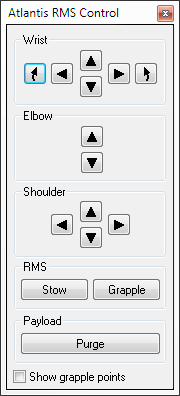
\includegraphics[width=0.2\hsize]{atlantis_rms_control.png}
\end{figure}

\noindent
The Shuttle carries a mechanical manipulator arm (SRMS, Shuttle Remote Manipulator System, also "Canadarm") in the cargo bay which can be used for releasing and recapturing satellites, deliver modules to the space station, as an MMU platform, etc.

The arm can be used in orbit once the cargo bay doors have been fully opened. Likewise, the arm must be stowed before the doors can be closed again.

In Orbiter, the arm is controlled with a dialog. Press \keystroke{Ctrl}\keystroke{Space} to bring up the Atlantis control box and select "RMS operation".

The arm has three joints: the shoulder joint can be rotated in yaw and pitch, the elbow joint can be rotated in pitch, and the wrist joint can be rotated in pitch, yaw and roll.

To grapple a satellite while stowed in the cargo bay, move the SRMS tip onto a grappling point and press "Grapple". If the satellite was successfully attached, the button label switches to "Release". To make it easier to identify the grappling points on the satellite, you can tick the "Show grapple points" box. This marks all grappling points with flashing arrows.

To release the satellite, press "Release".

You can also grapple freely drifting satellites if you move the SRMS tip onto a grappling point. To return a satellite back to Earth, it must be stowed in the cargo bay. Use the SRMS arm to bring the satellite into its correct stowing position in the payload bay. When the Payload "Arrest" button becomes active, the satellite can be fixed in the bay by pressing the button. It is automatically released from the SRMS tip.\\

The SRMS arm can be stowed in its transport position by pressing the SRMS "Stow" button. This is only possible as long as no object is attached to the arm. Payload can be released directly from the bay by pressing the "Purge" button.
\begin{center}
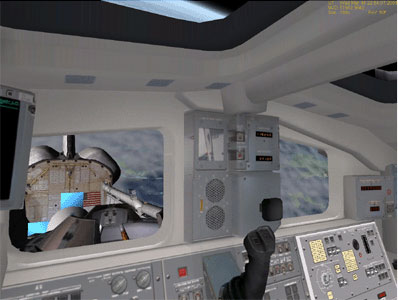
\includegraphics[width=0.6\textwidth]{atlantis_aft_flight_deck.jpg}
\captionof{figure}{View into the payload bay from the payload operator position.}
\end{center}

\subsubsection{Keyboard controls}
In addition to the generic Orbiter vessel control keys, Atlantis supports the following vessel-specific key controls:

\begin{table}[H]
	\centering
	\begin{tabular}{ |l|l| }
	\hline\rule{0pt}{2ex}
	\textbf{Shortcut} & \textbf{Action}\\
	\hline\rule{0pt}{2ex}
	\keystroke{G} & Operate landing gear (activated only after ET separation)\\
	\hline\rule{0pt}{2ex}
	\keystroke{J} & Jettison: separate SRBs or ET\\
	\hline\rule{0pt}{2ex}
	\keystroke{K} & Operate cargo bay doors (shortcut - for the full procedure see \ref{para:atlantis_baydoor})\\
	\hline\rule{0pt}{2ex}
	\keystroke{Ctrl}\keystroke{B} & Operate split-rudder brake\\
	\hline\rule{0pt}{2ex}
	\keystroke{Ctrl}\keystroke{U} & Deploy/retract Ku-band antenna (shortcut - for the full procedure see \ref{para:atlantis_antenna})\\
	\hline\rule{0pt}{2ex}
	\keystroke{Ctrl}\keystroke{Space} & Open control box for access to payload bay and SRMS control dialogs.\\
	\hline
	\end{tabular}
\end{table}

\subsubsection{Configuration}

\begin{figure}[H]
  \centering
  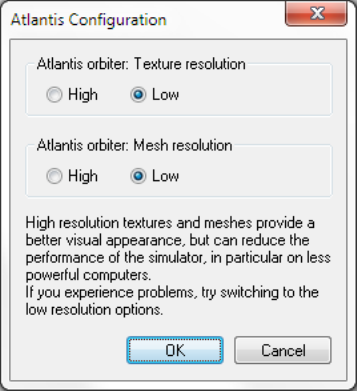
\includegraphics[width=0.4\hsize]{atlantis_config.png}
\end{figure}

\noindent
The Space Shuttle model included with the Orbiter distribution contains very detailed meshes and textures of the exterior and flightdeck interior to provide the best possible visual appearance. On some older computers this may lead to loss of performance and slow response. To address this problem, Orbiter can be configured to use a less detailed visual model.
On the Extra tab of the Orbiter Launchpad, double-click Vessel configuration, followed by Atlantis Configuration. Switch the Texture and Mesh resolution settings to Low. This will put less load on the graphics system of your computer, at the cost of some visual detail.

\subsubsection{Implementation notes}
This section contains details of the implementation of the Space Shuttle (Atlantis) vessel class in Orbiter. The C++ module code for the Shuttle orbiter, the external tank and the solid rocket boosters is available in the.$/Src/Vessel/Atlantis$ subdirectory of the Orbiter source distribution. The physical parameters discussed in this section are the values used by Orbiter, as collected from public sources or guessed from fitting flight parameters. They may in some cases deviate from the actual Space Shuttle specifications. Suggestions and corrections to the model are always welcome.

\paragraph{Mesh-derived parameters}
The following parameters were extracted from the surface meshes of the Shuttle components:

\begin{table}[H]
\centering
\begin{tabular}{|l|l|l|l|}
\hline
\multicolumn{4}{|l|}{\cellcolor{cyan!10}Orbiter}\\
\hline
Length & 39.16 & m & \\
\hline
Wingspan & 24.54 & m & \\
\hline
Height & 14.29 & m & \\
\hline
Volume & 1133 & m$^{3}$ & \\
\hline
Cross-sections & 234.8 / 389.1 / 68.2 & m$^{2}$ & (side-on / top-down / head-on)\\
\hline
PMI* & 78.2 / 82.1 / 10.7 & m$^{2}$ & (xx / yy / zz)\\
\hline
\multicolumn{4}{|l|}{\cellcolor{yellow!10}External tank (ET)}\\
\hline
Length & 47.83 & m & \\
\hline
Diameter & 9.68 & m & \\
\hline
Volume & 2829 & m$^{3}$ & \\
\hline
Cross-sections & 412.1 / 411.8 / 72.7 & m$^{2}$ & (side-on / top-down / head-on)\\
\hline
PMI* & 145.6 / 145.6 / 10.5 & m$^{2}$ & (xx / yy / zz)\\
\hline
\multicolumn{4}{|l|}{\cellcolor{cyan!10}Solid rocket booster (SRB)}\\
\hline
Length & 45.7 & m & \\
\hline
Diameter & 3.8 & m & \\
\hline
Volume & 452 & m$^{3}$ & \\
\hline
Cross-sections & 162.1 / 162.1 / 26.6 & m$^{2}$ & (side-on / top-down / head-on)\\
\hline
PMI* & 154.3 / 154.3 / 1.83 & m$^{2}$ & (xx / yy / zz)\\
\hline
\multicolumn{4}{|l|}{\cellcolor{yellow!10}Orbiter + ET assembly}\\
\hline
Length & 57.55 & m & \\
\hline
Height & 24.44 & m & \\
\hline
Volume & 3962 & m$^{3}$ & \\
\hline
Cross-sections & 646.2 / 597.5 / 140.0 & m$^{2}$ & (side-on / top-down / head-on)\\
\hline
PMI* & 173.3 / 161.0 / 24.0 & m$^{2}$ & (xx / yy / zz)\\
\hline
\multicolumn{4}{|l|}{\cellcolor{cyan!10}Orbiter + ET + SRBs (launch assembly)}\\
\hline
Length & 57.91 & m & \\
\hline
Height & 24.44 & m & \\
\hline
Volume & 4868 & m$^{3}$ & \\
\hline
Cross-sections & 687.4 / 849.5 / 189.4 & m$^{2}$ & (side-on / top-down / head-on)\\
\hline
PMI* & 179.1 / 176.8 / 29.3 & m$^{2}$ & (xx / yy / zz)\\
\hline
\end{tabular}
\end{table}
\noindent
\textit{*:	PMI (principal moments of inertia, diagonal elements of inertia tensor, mass-normalised, assuming homogeneous density distribution}\\
\textit{**:	ET dimensions including Orbiter mounting brackets}

\paragraph{SRB thrust characteristics}
The following parameters are used for the solid rocket boosters (per unit):

\begin{table}[H]
\centering
\begin{tabular}{|l|l|l|l|}
\hline
Thrust at liftoff & 11791.8 & kN & \\
\hline
Weight empty & 87543 & kg & \\
\hline
Weight propellant & 502126 & kg & \\
\hline
SRB separation & 126 & s & after liftoff\\
\hline
\end{tabular}
\end{table}

The SRB thrust rate is modelled as a piecewise linear function. The assumed thrust rate and resulting remaining propellant are listed in the following table as a percentage (liftoff time t = 0):

\begin{table}[H]
\centering
\begin{tabular}{|l|l|l|l|l|l|l|}
\hline
Time[s] 	 			& -4  & -1     & 103    & 115   & 126 (sep) & 135 \\
\hline
Thrust[\%] 			& 0   & 100    & 100    & 85    & 5         & 0   \\
\hline
Propellant[\%]  & 100 & 98.768 & 13.365 & 4.250 & 0.185     & 0   \\
\hline
\end{tabular}
\end{table}

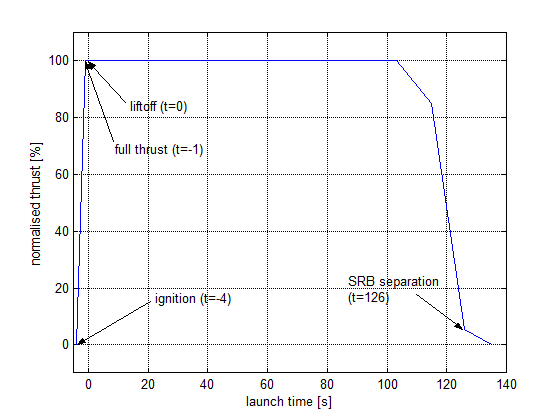
\includegraphics[width=0.5\linewidth]{atlantis_srb_thrust.png}
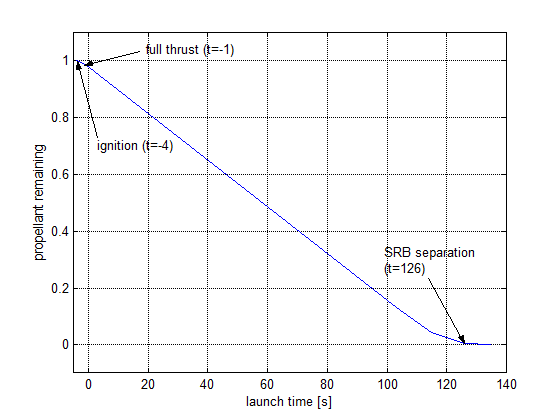
\includegraphics[width=0.5\linewidth]{atlantis_srb_prop.png}

The value derived from this table for specific impulse (Isp), i.e. the amount of thrust obtained from burning 1 kg of propellant per second, is
$I_{sp} = 2859.74 m/s$
The actual maximum thrust also depends on the ambient atmospheric pressure. The model assumes freespace thrust to be 1.25 × the thrust at liftoff at sea level, with an exponential pressure relationship of the following form:
\begin{center}
\[F = F_\infty e^{-p\beta}\] with \[\beta = -\frac{1}{p_0\ln{(F_0/F_\infty)}}\]
\end{center}
where $p_0$ is the pressure at liftoff altitude, $p$ is the current pressure, and $F_0$ and $F_\infty$ are the liftoff and freespace thrust values, respectively.

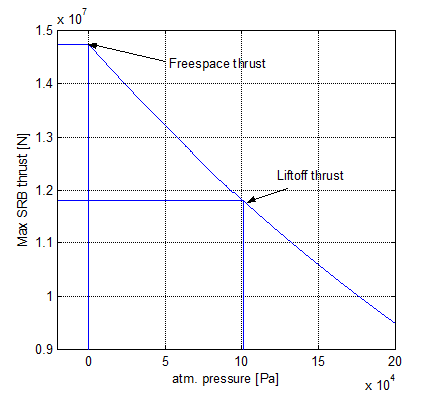
\includegraphics[width=0.5\linewidth]{atlantis_srb_atm.png}

\noindent
Problems:
\begin{itemize}
\item The thrust curve during the burnout stage is not based on any data. In particular the amount of thrust produced at separation (t = 126s) is not known.
\item According to sources, the SRBs reduce thrust by $1/3$ after 50s to keep acceleration within limits. This is not currently modelled.
\item The pressure-thrust relationship is assumed, not backed by any data.
\end{itemize}

\paragraph{Orbiter aerodynamic characteristics}
The Atlantis orbiter uses the following subsonic lift and moment coefficients:\\

\textbf{\large Vertical lift component - wings and body}\\

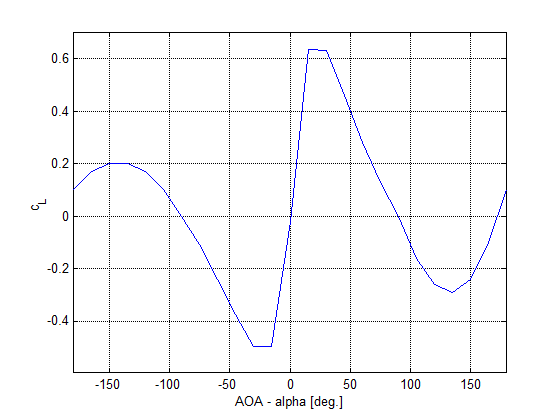
\includegraphics[width=0.5\linewidth]{atlantis_aero_v_aoa_cl.png}
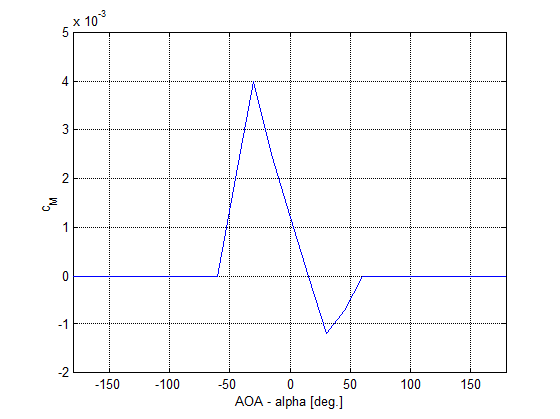
\includegraphics[width=0.5\linewidth]{atlantis_aero_v_aoa_cm.png}

The lift profile utilises a documented lift slope of 0.0437/deg. Everything else is assumed. In particular the moment coefficient profile needs more thought. Other parameters:

\begin{table}[H]
\centering
\begin{tabular}{|l|l|}
\hline
Zero-lift drag & $c_{D,0}$ = $0.06$ \\ \hline
Chord length & $c$ = $20 m$ \\ \hline
Reference area & $S$ = $270 m^2$ \\ \hline
Wing aspect ratio & $A$ = $2.266$ \\ \hline
Oswald efficiency factor & $e_0$ = $0.6$ \\ \hline
\end{tabular}
\end{table}

\begin{center}
This produces the following drag polar:

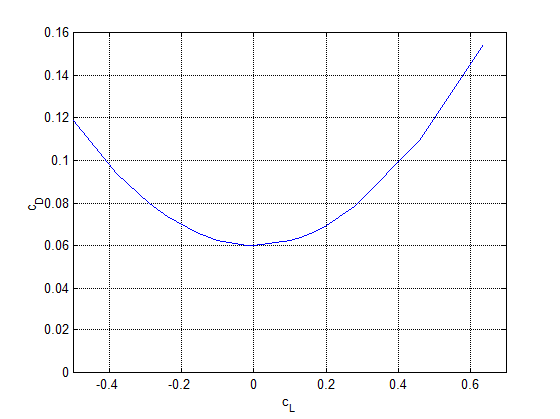
\includegraphics[width=0.5\linewidth]{atlantis_aero_v_cl_cd.png}
\end{center}

\textbf{\large Horizontal lift component - vertical stabiliser and body}\\

Lift coefficient and drag polar for the horizontal lift component (produced by the orbiter body and vertical stabiliser) are given by:

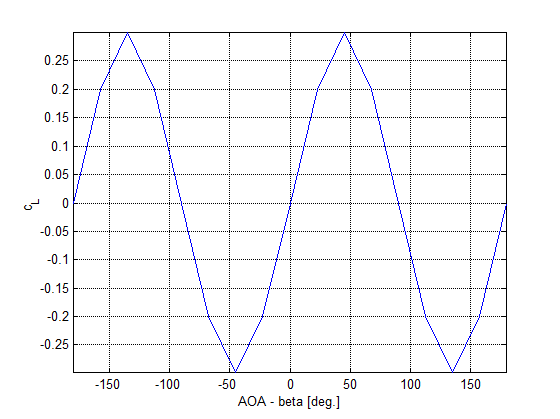
\includegraphics[width=0.5\linewidth]{atlantis_aero_h_aoa_cl.png}
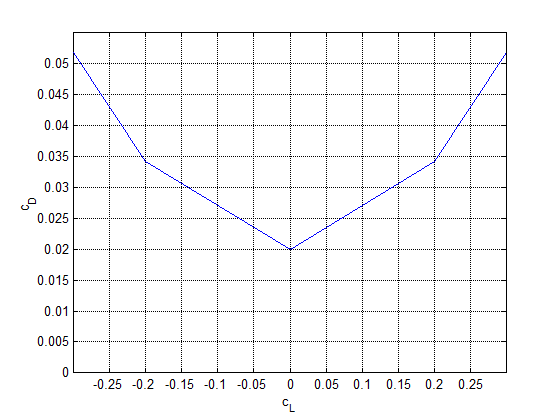
\includegraphics[width=0.5\linewidth]{atlantis_aero_h_cl_cd.png}

The horizontal lift profile is symmetric (symmetric airfoil). Other parameters:

\begin{table}[H]
\centering
\begin{tabular}{|l|l|}
\hline
Moment coefficient & $c_M$ = $0$ \\ \hline
Zero-lift drag & $c_{D,0}$ = $0.02$ \\ \hline
Chord length & $c$ = $20 m$ \\ \hline
Reference area & $S$ = $50 m^2$ \\ \hline
Wing aspect ratio & $A$ = $1.5$ \\ \hline
Oswald efficiency factor & $e_0$ = $0.6$ \\ \hline
\end{tabular}
\end{table}

\textbf{\large Speed brake}\\

The split-rudder speed brake is activated with \keystroke{Ctrl}\keystroke{B}. Deployment time is 4.93s. At full extent, the brake generates a subsonic drag force of 5.0m$^{2}$ $q_\infty$ ($q_\infty$: freestream dynamic pressure) in Orbiter. It also generates a pitch-up moment.

\subsubsection{Credits}
The Atlantis orbiter 3-D model and virtual cockpit for the latest version of Orbiter has been kindly contributed by Michael Grosberg.\\

Don Gallagher's extensive work on the cockpit interior, including high resolution instrument panels, switches and buttons, was essential to realise the working virtual cockpit implementation.\\

Damir Gulesich has provided the models for the external tank (ET) and solid rocket boosters (SRB).\\

Robert Conley's code provided the basis for the RMS operation, and he also contributed the MMU extensions.\\

Douglas Beachy contributed the virtual cockpit code.\\

And not least I would like to thank the beta team for their valuable feedback during the development of the model and code.

\end{document}